%!TEX root = ../thesis.tex

\thispagestyle{myheadings}

\graphicspath{{Body/Figures/RatioAnalysis/}{Body/Figures/RatioAnalysis/MethodOverview/}}

\chapter{\texorpdfstring{\wa}{wa} Measurement}
\label{chapter:SpinPrecessionMeasurement}


The measurement of \wa is determined by counting the number of detected positrons in the calorimeters above some energy threshold, as described in \secref{section:WaIntro}. Doing so results in a histogram of counts which is modulated by \wa, \figref{fig:gm2wiggle}. Fitting for the frequency allows \wa to be extracted. The \wa measurement therefore consists of the steps needed to construct the histogram of counts, and the fitting of said histogram.


\section{Reconstruction}
\label{sec:ReconWest}


The calorimeters measure hit times and energies of impacting particles, where these hit times and energies are determined from SiPM current signals and a reconstruction procedure. The reconstruction procedure consists of the steps need to take the raw signals and produce correct measurements of the positron energies and times. In E989 there are two separate reconstruction algorithms, \texttt{ReconWest} and \texttt{ReconEast}. Using separate reconstruction methods gives confidence in any final results be removing any single points of failure. The reconstruction method used in this analysis is \texttt{ReconWest}. A summary of its details will be presented here. A more thorough description is detailed by A. Fienberg \cite{AFThesis}.


The raw data are digitized waveforms, which are voltage versus time signals output from each SiPM. Due to the incredible amount of data coming in with the high muon fill rate, only those traces which exceed some threshold are saved to disk. An online processing system checks the traces against this preconfigured threshold by passing all of the data through a GPU farm \cite{Gohn:2016shi}. If any trace is found above threshold, then the data is saved from every SiPM in every calorimeter, for a time range around the over-threshold pulse. This time range is called a time island, similar to in the tracking reconstruction, and typically has a width of $\SI{40}{ns}$ \cite{AFThesis}.






-clockticks






-overview of reconstruction

-need to mention gain


-clustering




\section{Histogramming}
\label{sec:Histogramming}


Once the reconstruction has processed all the hits into clusters, the time spectra histograms need to be made.



-artificial deadtime
-time randomization

-here or maybe in a later section mention the pileup procedure, maybe a subsection


\section{Lost muons}
\label{sec:lostmuons}

\section{Fitting}
\label{sec:Fitting}


-detail the ratio method - might need to pull stuff out from my appendix


    \begin{figure}[]
    \centering
        \begin{subfigure}[t]{0.45\textwidth}
            \centering
            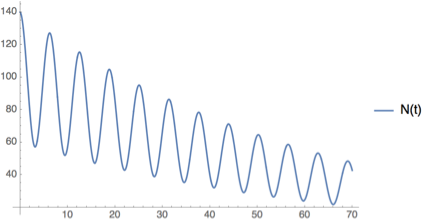
\includegraphics[width=\textwidth]{FiveParamFunc}
            \caption{}
        \end{subfigure}%

        \vspace{2mm}
        \begin{subfigure}[t]{0.45\textwidth}
            \centering
            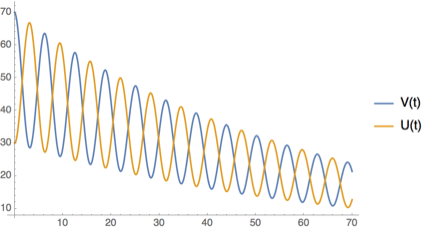
\includegraphics[width=\textwidth]{UVFuncs}
            \caption{}
        \end{subfigure}
        \begin{subfigure}[t]{0.45\textwidth}
            \centering
            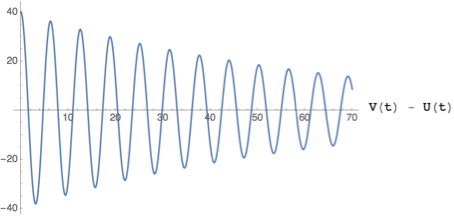
\includegraphics[width=\textwidth]{RatioNumFunc}
            \caption{}
        \end{subfigure}%
        \vspace{2mm}
        \begin{subfigure}[t]{0.45\textwidth}
            \centering
            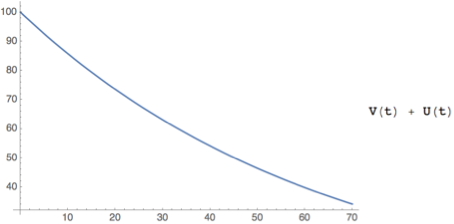
\includegraphics[width=\textwidth]{RatioDenomFunc}
            \caption{}
        \end{subfigure}
        \begin{subfigure}[t]{0.45\textwidth}
            \centering
            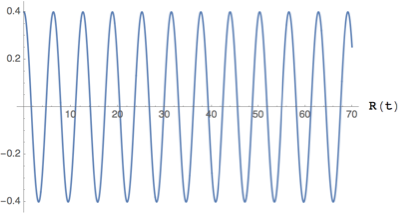
\includegraphics[width=\textwidth]{RatioFunc}
            \caption{}
        \end{subfigure}% 
    \caption[]{}
    \label{}
    \end{figure}






\section{Systematic errors}
\label{sec:Systematic Errors}



\cleardoublepage
